\subsection*{Resultater}
Resultater har to boundarys, hvortil der er opstillet en controlklasse. Boundarys og tilhørende controller fremgår af \autoref{fig:MVCresultater}. 

\begin{figure} [H]
\centering
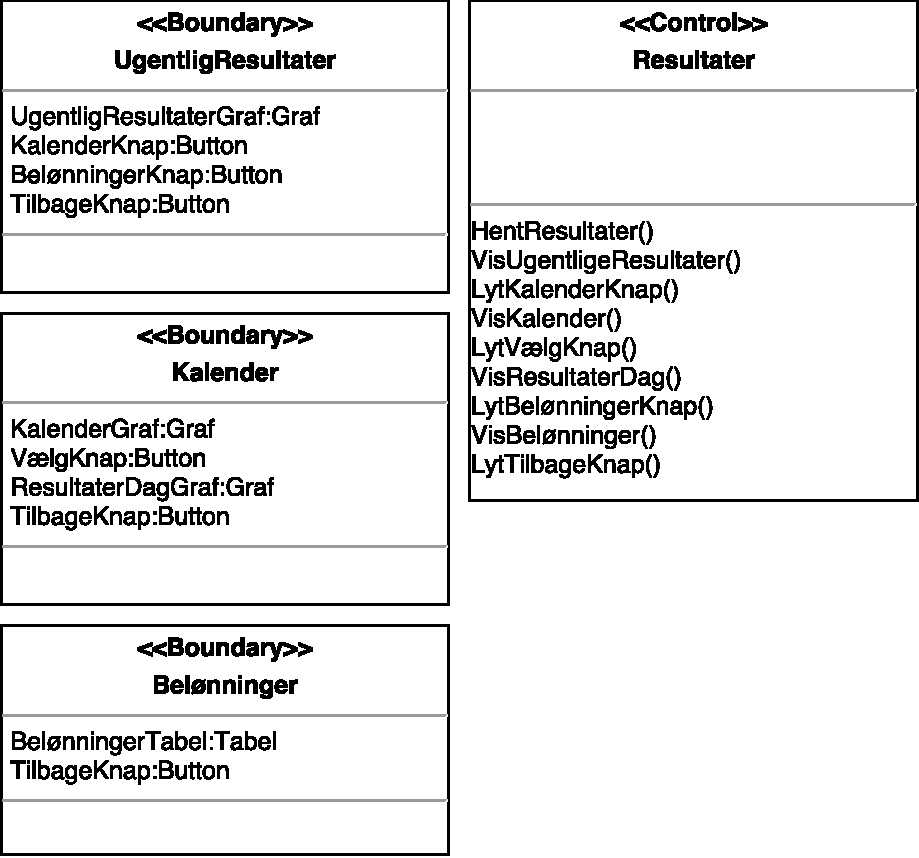
\includegraphics[width=1\textwidth]{figures/MVC/MVCResultater}
\caption{Designklasser for resultater. Til venstre ses boundarys for den grafiske udvikling og belønninger. Til højre fremgår den tilhørende controller.}
\label{fig:MVCresultater}
\end{figure}

\noindent
I grænsefladen for \textit{GrafiskUdvikling} er der opstillet en graf af typen BarChart samt en knap af typen Button, for at give mulighed for at tilgå belønninger. Boundary for \textit{Belønninger} indeholder billeder af typen ImageView og tekstfelter af typen TextView. Billederne viser antallet af stjerner, der repræsenterer belønninger, brugeren har opnået.
\textit{Resultater}-controlleren indeholder attributter og metoder. Disse metoder omfatter Hent, Vis, Lyt og Start. Der er er opstillet attributter, hvoraf to af disse er af typen ArrayList, der benyttes til at lagre resultater samt belønninger. Hent-metoder handler ud fra definerede inputsparametre og er angivet void. 

I sammenspil med designklasserne for resultater er der udarbejdet et sekvensdiagram, hvilket fremgår af \autoref{fig:SEKResultater}

\begin{figure} [H]
\centering
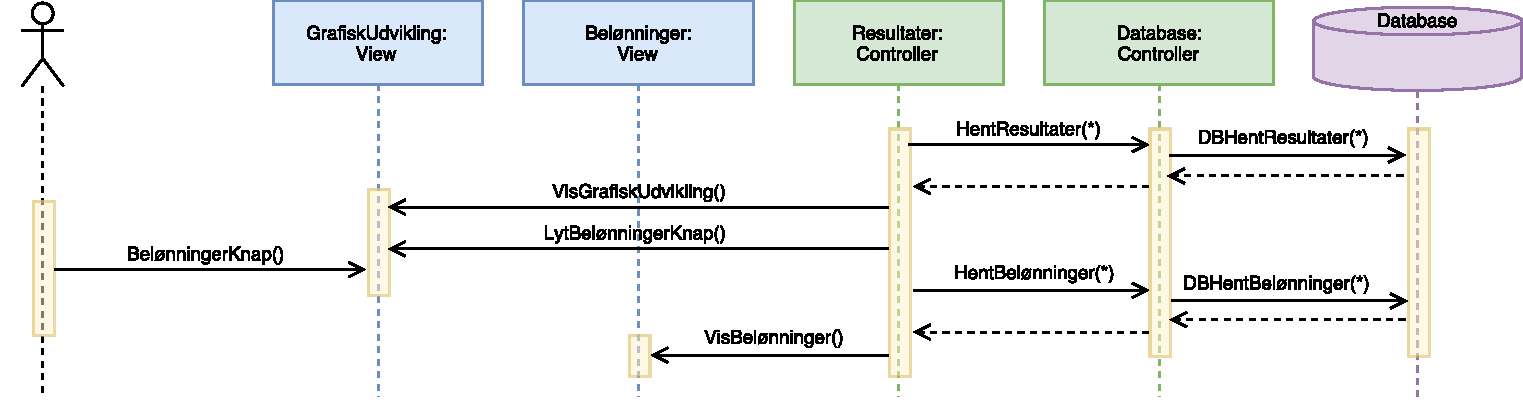
\includegraphics[width=1\textwidth]{figures/Sek/SEKResultater}
\caption{Sekvensdiagram for Resultater.}
\label{fig:SEKResultater}
\end{figure} 

\noindent 
Når brugeren tilgår resultater, henter \textit{Resultat}-controller, gennem \textit{Database}-controller, brugerens resultater fra \textit{Database}. Resultater vises i et BarChart i grænsefladen for \textit{GrafiskUdvikling}. Dertil er der opstillet en BelønningerKnap, der videresender brugeren til grænsefladen for \textit{Belønninger} ved tryk. Idet brugeren trykker på knappen, henter \textit{Resultat}-controller, gennem \textit{Database}-controller, brugerens belønninger, der vises i grænsefladen. Denne viser stjerner opnået indenfor tid, afstand, konditonstræning og antal træninger.

%Der er til \textit{ResultaterGrænseflade} opstillet en \textit{ResultatController}, der har til formål at hente nye resultater fra dagens træning i træningscontrolleren, når resultater tilgås via hovedmenugrænsefladen. Herefter vises en oversigtsgraf over udført træning. Træningscontrolleren fremgår af \autoref{fig:MVCTraening}.
%Controlleren lytter på om brugeren trykker på de angivne knapper i grænsefladen for resultater og viser valgt handling, hvis dette er tilfældet. 
